\documentclass{standalone}
\usepackage{tikz}
\usetikzlibrary{positioning, arrows.meta, calc, shapes.multipart}

\begin{document}

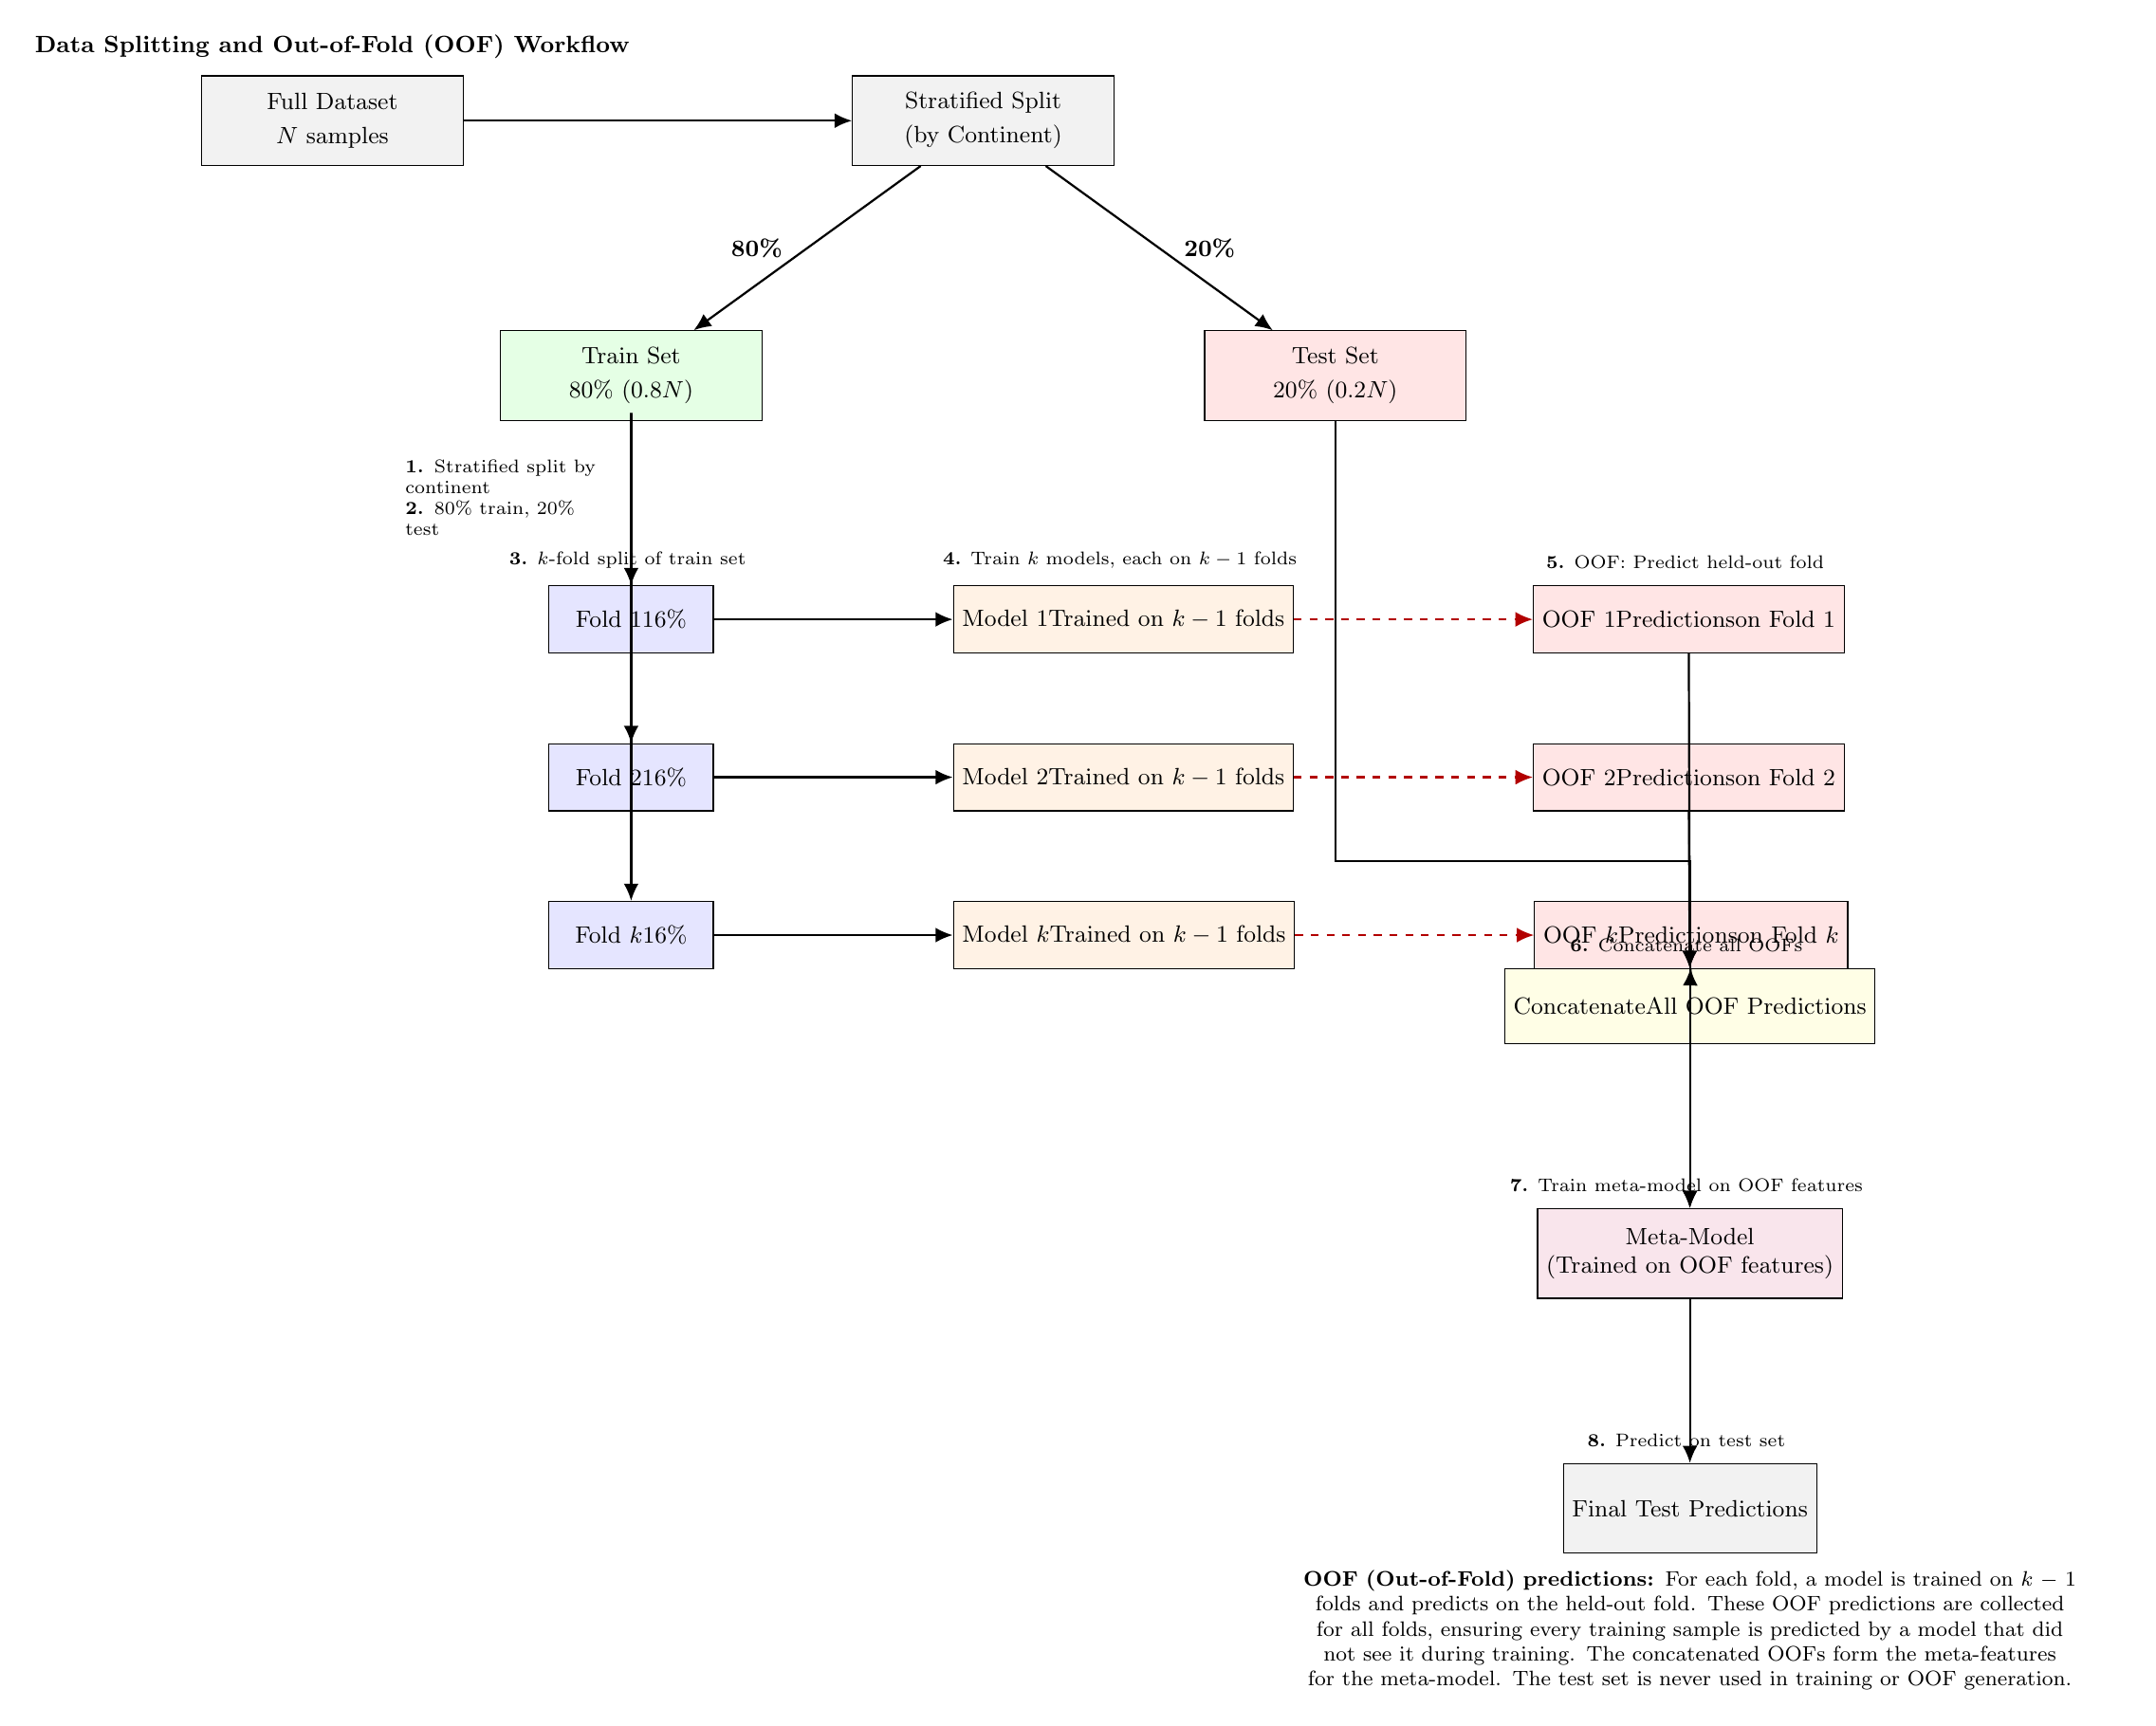
\begin{tikzpicture}[
    block/.style={rectangle, draw, minimum height=1.2cm, minimum width=3.5cm, align=center, fill=gray!10},
    fold/.style={rectangle, draw, minimum height=0.9cm, minimum width=2.2cm, fill=blue!10},
    model/.style={rectangle, draw, minimum height=0.9cm, minimum width=2.2cm, fill=orange!10},
    oof/.style={rectangle, draw, minimum height=0.9cm, minimum width=2.2cm, fill=red!10},
    concat/.style={rectangle, draw, minimum height=1.0cm, minimum width=3.2cm, fill=yellow!10},
    arrow/.style={-{Latex[width=2mm]}, thick},
    dashedarrow/.style={dashed, -{Latex[width=2mm]}, thick, color=red!70!black},
    every node/.style={font=\small}
]

% Full dataset
\node[block] (data) {Full Dataset\\[2pt] $N$ samples};

% Train/Test split
\node[block, right=5.2cm of data] (split) {Stratified Split\\[2pt] (by Continent)};

\draw[arrow] (data) -- (split);

% Train/Test blocks with proportions
\node[block, below left=2.2cm and 1.2cm of split, fill=green!10] (train) {Train Set\\[2pt] $80\%$ ($0.8N$)};
\node[block, below right=2.2cm and 1.2cm of split, fill=red!10] (test) {Test Set\\[2pt] $20\%$ ($0.2N$)};

\draw[arrow] (split) -- node[left, xshift=-0.2cm] {\textbf{80\%}} (train);
\draw[arrow] (split) -- node[right, xshift=0.2cm] {\textbf{20\%}} (test);

% Arrange folds vertically
\node[fold, below=2.2cm of train, xshift=0cm] (fold1) {Fold 1\\$16\%$};
\node[fold, below=1.2cm of fold1] (fold2) {Fold 2\\$16\%$};
\node[fold, below=1.2cm of fold2] (foldk) {Fold $k$\\$16\%$};

\draw[arrow] (train) -- (fold1);
\draw[arrow] (train) -- ++(0,-0.5) -| (fold2);
\draw[arrow] (train) -- ++(0,-1.5) -| (foldk);

% Models vertically aligned to folds
\node[model, right=3.2cm of fold1] (model1) {Model 1\\Trained on $k-1$ folds};
\node[model, right=3.2cm of fold2] (model2) {Model 2\\Trained on $k-1$ folds};
\node[model, right=3.2cm of foldk] (modelk) {Model $k$\\Trained on $k-1$ folds};

\draw[arrow] (fold1) -- (model1);
\draw[arrow] (fold2) -- (model2);
\draw[arrow] (foldk) -- (modelk);

% OOF predictions vertically aligned to models
\node[oof, right=3.2cm of model1] (oof1) {OOF 1\\Predictions\\on Fold 1};
\node[oof, right=3.2cm of model2] (oof2) {OOF 2\\Predictions\\on Fold 2};
\node[oof, right=3.2cm of modelk] (oofk) {OOF $k$\\Predictions\\on Fold $k$};

\draw[dashedarrow] (model1) -- (oof1);
\draw[dashedarrow] (model2) -- (oof2);
\draw[dashedarrow] (modelk) -- (oofk);

% Concatenate OOFs (centered below OOFs)
\node[concat, below=1.5cm of $(oof2)!0.5!(oofk)$] (concat) {Concatenate\\All OOF Predictions};

\draw[arrow] (oof1) -- (concat);
\draw[arrow] (oof2) -- (concat);
\draw[arrow] (oofk) -- (concat);

% Meta-model
\node[block, below=2.2cm of concat, fill=purple!10] (meta) {Meta-Model\\(Trained on OOF features)};

\draw[arrow] (concat) -- (meta);

% Final test prediction
\draw[arrow] (test) -- ++(0,-6.5) -| (meta);

\node[block, below=2.2cm of meta, minimum width=3.2cm] (final) {Final Test Predictions};

\draw[arrow] (meta) -- (final);

% Labels and explanations
\node[above=0.1cm of data] {\textbf{Data Splitting and Out-of-Fold (OOF) Workflow}};
\node[below=0.1cm of final, align=center, font=\footnotesize, text width=0.95\linewidth] {
    \textbf{OOF (Out-of-Fold) predictions:} For each fold, a model is trained on $k-1$ folds and predicts on the held-out fold. These OOF predictions are collected for all folds, ensuring every training sample is predicted by a model that did not see it during training. The concatenated OOFs form the meta-features for the meta-model. The test set is never used in training or OOF generation.
};

% Step annotations
\node[align=left, font=\scriptsize, left=0.2cm of train, anchor=east, text width=2.7cm] at ($(train)!0.5!(fold1)$) {%
    \textbf{1.} Stratified split by continent\\
    \textbf{2.} $80\%$ train, $20\%$ test
};
\node[align=left, font=\scriptsize, above=0.1cm of fold1, anchor=south] {%
    \textbf{3.} $k$-fold split of train set
};
\node[align=left, font=\scriptsize, above=0.1cm of model1, anchor=south] {%
    \textbf{4.} Train $k$ models, each on $k-1$ folds
};
\node[align=left, font=\scriptsize, above=0.1cm of oof1, anchor=south] {%
    \textbf{5.} OOF: Predict held-out fold
};
\node[align=left, font=\scriptsize, above=0.1cm of concat, anchor=south] {%
    \textbf{6.} Concatenate all OOFs
};
\node[align=left, font=\scriptsize, above=0.1cm of meta, anchor=south] {%
    \textbf{7.} Train meta-model on OOF features
};
\node[align=left, font=\scriptsize, above=0.1cm of final, anchor=south] {%
    \textbf{8.} Predict on test set
};

\end{tikzpicture}

\end{document}
\end{document}
